\documentclass[a4paper,14pt]{extreport} % формат документа

\usepackage{amsmath}
\usepackage{cmap} % поиск в ПДФ
\usepackage[T2A]{fontenc} % кодировка
\usepackage[utf8]{inputenc} % кодировка исходного текста
\usepackage[english,russian]{babel} % локализация и переносы
\usepackage[left = 2cm, right = 1cm, top = 2cm, bottom = 2 cm]{geometry} % поля
\usepackage{listings}
\usepackage{graphicx} % для вставки рисунков
\usepackage{amsmath}
\usepackage{float}
\usepackage{multirow}
\graphicspath{{images/}}
\DeclareGraphicsExtensions{.pdf,.png,.jpg}
\newcommand{\anonsection}[1]{\section*{#1}\addcontentsline{toc}{section}{#1}}

\lstset{ %
	language=C,                % Язык программирования 
	numbers=left,                   % С какой стороны нумеровать          
	frame=single,                    % Добавить рамку
	basicstyle=\small,
    escapebegin=\begin{russian}\commentfont,
    escapeend=\end{russian},
    literate={Ö}{{\"O}}1
    {Ä}{{\"A}}1
    {Ü}{{\"U}}1
    {ß}{{\ss}}1
    {ü}{{\"u}}1
    {ä}{{\"a}}1
    {ö}{{\"o}}1
    {~}{{\textasciitilde}}1
    {а}{{\selectfont\char224}}1
    {б}{{\selectfont\char225}}1
    {в}{{\selectfont\char226}}1
    {г}{{\selectfont\char227}}1
    {д}{{\selectfont\char228}}1
    {е}{{\selectfont\char229}}1
    {ё}{{\"e}}1
    {ж}{{\selectfont\char230}}1
    {з}{{\selectfont\char231}}1
    {и}{{\selectfont\char232}}1
    {й}{{\selectfont\char233}}1
    {к}{{\selectfont\char234}}1
    {л}{{\selectfont\char235}}1
    {м}{{\selectfont\char236}}1
    {н}{{\selectfont\char237}}1
    {о}{{\selectfont\char238}}1
    {п}{{\selectfont\char239}}1
    {р}{{\selectfont\char240}}1
    {с}{{\selectfont\char241}}1
    {т}{{\selectfont\char242}}1
    {у}{{\selectfont\char243}}1
    {ф}{{\selectfont\char244}}1
    {х}{{\selectfont\char245}}1
    {ц}{{\selectfont\char246}}1
    {ч}{{\selectfont\char247}}1
    {ш}{{\selectfont\char248}}1
    {щ}{{\selectfont\char249}}1
    {ъ}{{\selectfont\char250}}1
    {ы}{{\selectfont\char251}}1
    {ь}{{\selectfont\char252}}1
    {э}{{\selectfont\char253}}1
    {ю}{{\selectfont\char254}}1
    {я}{{\selectfont\char255}}1
    {А}{{\selectfont\char192}}1
    {Б}{{\selectfont\char193}}1
    {В}{{\selectfont\char194}}1
    {Г}{{\selectfont\char195}}1
    {Д}{{\selectfont\char196}}1
    {Е}{{\selectfont\char197}}1
    {Ё}{{\"E}}1
    {Ж}{{\selectfont\char198}}1
    {З}{{\selectfont\char199}}1
    {И}{{\selectfont\char200}}1
    {Й}{{\selectfont\char201}}1
    {К}{{\selectfont\char202}}1
    {Л}{{\selectfont\char203}}1
    {М}{{\selectfont\char204}}1
    {Н}{{\selectfont\char205}}1
    {О}{{\selectfont\char206}}1
    {П}{{\selectfont\char207}}1
    {Р}{{\selectfont\char208}}1
    {С}{{\selectfont\char209}}1
    {Т}{{\selectfont\char210}}1
    {У}{{\selectfont\char211}}1
    {Ф}{{\selectfont\char212}}1
    {Х}{{\selectfont\char213}}1
    {Ц}{{\selectfont\char214}}1
    {Ч}{{\selectfont\char215}}1
    {Ш}{{\selectfont\char216}}1
    {Щ}{{\selectfont\char217}}1
    {Ъ}{{\selectfont\char218}}1
    {Ы}{{\selectfont\char219}}1
    {Ь}{{\selectfont\char220}}1
    {Э}{{\selectfont\char221}}1
    {Ю}{{\selectfont\char222}}1
    {Я}{{\selectfont\char223}}1
    {і}{{\selectfont\char105}}1
    {ї}{{\selectfont\char168}}1
    {є}{{\selectfont\char185}}1
    {ґ}{{\selectfont\char160}}1
    {І}{{\selectfont\char73}}1
    {Ї}{{\selectfont\char136}}1
    {Є}{{\selectfont\char153}}1
    {Ґ}{{\selectfont\char128}}1
}

\begin{document}
\begin{titlepage}

    \begin{table}[H]
        \centering
        \footnotesize
        \begin{tabular}{cc}
            \multirow{8}{*}{\includegraphics[scale=0.35]{bmstu.jpg}}
            & \\
            & \\
            & \textbf{Министерство науки и высшего образования Российской Федерации} \\
            & \textbf{Федеральное государственное бюджетное образовательное учреждение} \\
            & \textbf{высшего образования} \\
            & \textbf{<<Московский государственный технический} \\
            & \textbf{университет имени Н.Э. Баумана>>} \\
            & \textbf{(МГТУ им. Н.Э. Баумана)} \\
        \end{tabular}
    \end{table}

    \vspace{-2.5cm}

    \begin{flushleft}
        \rule[-1cm]{\textwidth}{3pt}
        \rule{\textwidth}{1pt}
    \end{flushleft}

    \begin{flushleft}
        \small
        ФАКУЛЬТЕТ
        \underline{<<Информатика и системы управления>>\ \ \ \ \ \ \ 
        \ \ \ \ \ \ \ \ \ \ \ \ \ \ \ \ \ \ \ \ \ \ \ \ \ \ \ \ \ \ \ 
    \ \ \ \ \ \ \ \ \ \ \ \ \ \ \ } \\
        КАФЕДРА
        \underline{<<Программное обеспечение ЭВМ и
        информационные технологии>>
        \ \ \ \ \ \ \ \ \ \ \ \ \ \ \ \ \ \ \ \ }
    \end{flushleft}

    \vspace{2cm}

    \begin{center}
        \textbf{Лабораторная работа № 3} \\
        \vspace{0.5cm}
    \end{center}

    \vspace{4cm}

    \begin{flushleft}
        \begin{tabular}{ll}
            \textbf{Дисциплина} & Операционные системы.  \\
            \textbf{Тема} & Загружаемые модули ядра.  \\
            \\
            \textbf{Студент} & Сиденко А.Г. \\
            \textbf{Группа} & ИУ7-63Б \\
            \textbf{Оценка (баллы)} & \\
            \textbf{Преподаватель} & Рязанова Н.Ю.   \\
        \end{tabular}
    \end{flushleft}

    \vspace{4cm}

   \begin{center}
        Москва, 2020 г.
    \end{center}

\end{titlepage}

\textbf{Пример простого загружаемого модуля ядра} 

\begin{lstlisting}
#include <linux/init.h>
#include <linux/module.h>
#include <linux/kernel.h>

MODULE_LICENSE("GPL");
MODULE_AUTHOR("Sidenko");
MODULE_DESCRIPTION("Lab3");

// Инициализация модуля
static int __init my_module_init(void)
{
   printk(KERN_INFO "Start!\n");
   return 0;
}

// Удаление модуля
static void __exit my_module_exit(void)
{
   printk(KERN_INFO "End!\n");
}

module_init(my_module_init);
module_exit(my_module_exit);
\end{lstlisting}

\begin{enumerate}

\item Загрузка и выгрузка модуля ядра:

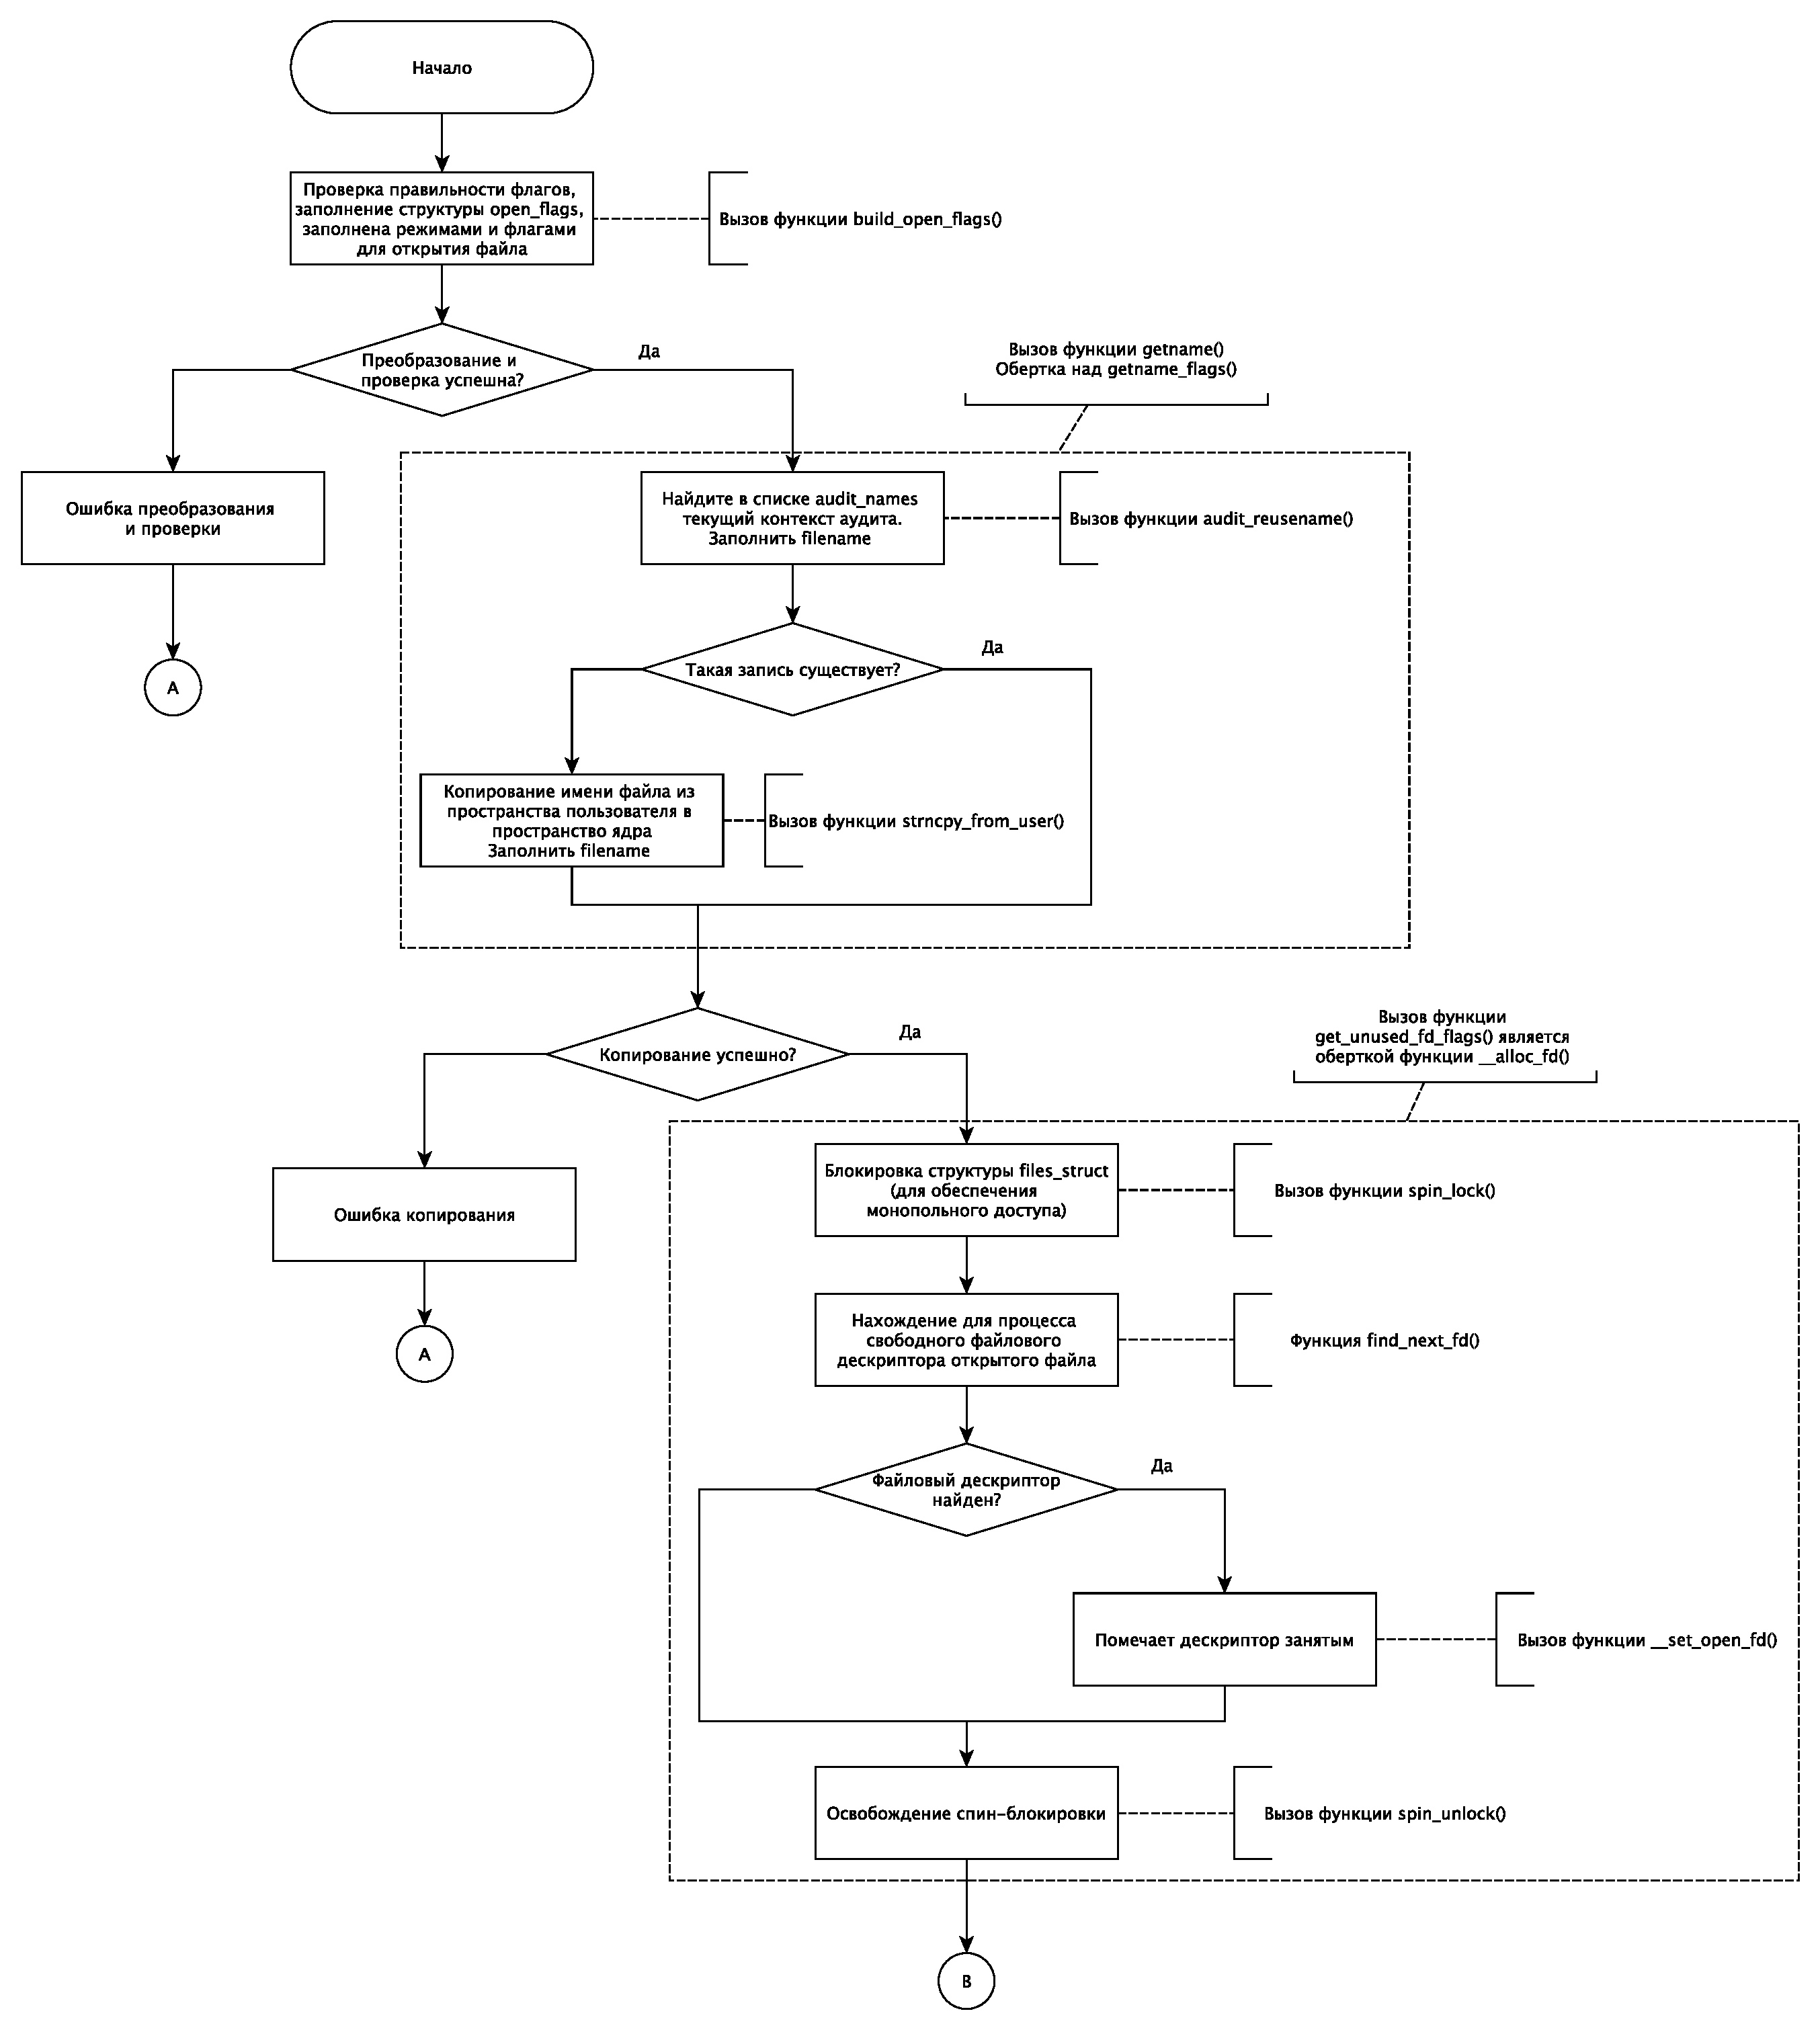
\includegraphics[scale=0.45]{1}

\item Вывод буфера сообщений ядра в стандартный поток вывода:

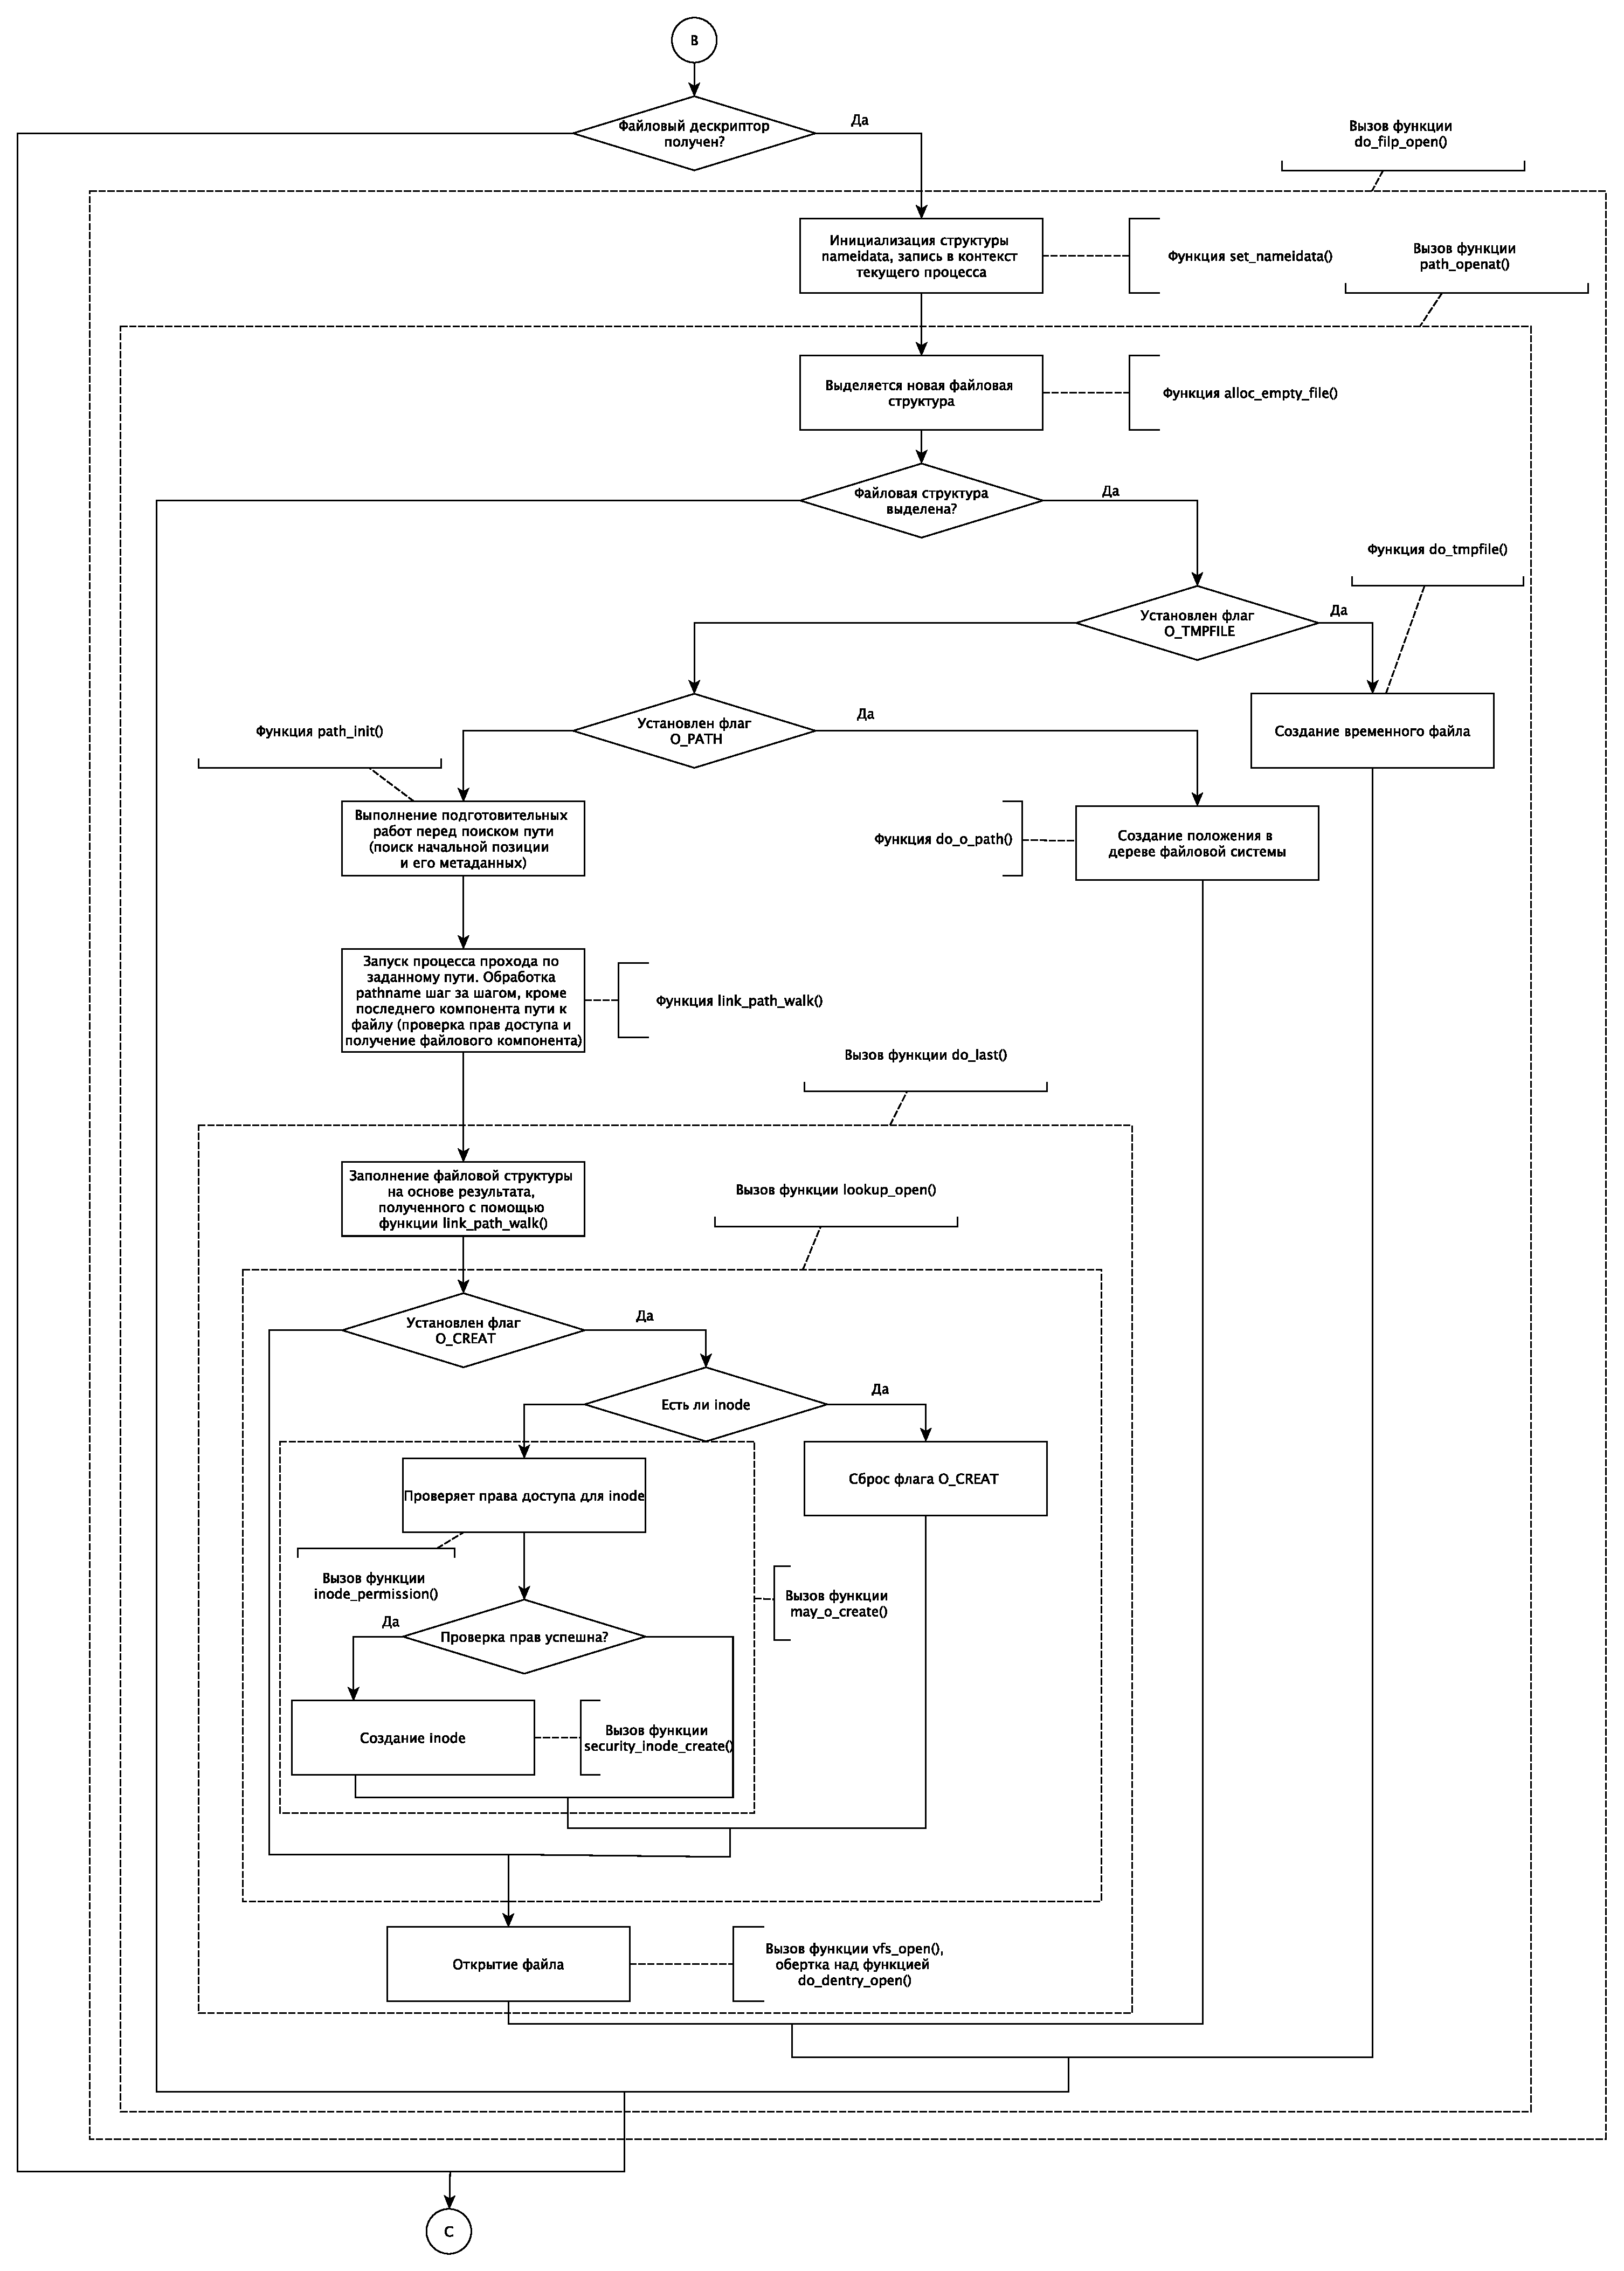
\includegraphics[scale=0.45]{2}
\end{enumerate}

\newpage

\textbf{Модуль md1}

Модуль md1 демонстрирует возможность создания экспортируемых данных и функций.

\begin{lstlisting}
#include <linux/init.h>
#include <linux/module.h>
#include "md.h"

MODULE_LICENSE("GPL");
MODULE_AUTHOR("Sidenko");
MODULE_DESCRIPTION("Lab3");

char* md1_str_data = "Привет из модуля 1!";
int md1_int_data = 111;

extern char* md1_get_str(int n)
{
  printk(KERN_INFO "MODULE1: md1_get_str(%d) called\n", n);
  switch (n)
  {
  case 1:
    return "Привет!";
    break;
  case 2:
    return "Пока!";
    break;
  default:
    return "Передайте 1 для приветствия или 2 для прощания";
    break;
  }
}

extern int md1_factorial(int n)
{
  printk(KERN_INFO "MODULE1: md1_factorial(%d) called\n", n);

  int i, answer = 1;

  if (n <= 0)
    return 0;

  for (i = 2; i <= n; i++)
    answer *= i;

  return answer;
}

// экспортируем данные
EXPORT_SYMBOL(md1_str_data);
EXPORT_SYMBOL(md1_int_data);
// экспортируем функции
EXPORT_SYMBOL(md1_get_str);
EXPORT_SYMBOL(md1_factorial);

static int __init my_module_init(void)
{
  printk(KERN_INFO "MODULE1: loaded\n");
  return 0;
}

static void __exit my_module_exit(void)
{
  printk(KERN_INFO "MODULE1: unloaded\n");
}

module_init(my_module_init);
module_exit(my_module_exit);
\end{lstlisting}

\textbf{Модуль md2}

Модуль md2 демонстрирует использование данных и функций экспортируемых первым модулем (md1).

\begin{lstlisting}
#include <linux/init.h>
#include <linux/module.h>
#include "md.h"

MODULE_LICENSE("GPL");
MODULE_AUTHOR("Sidenko");
MODULE_DESCRIPTION("Lab3");

static int __init my_module_init(void)
{
  printk(KERN_INFO "MODULE2: loaded\n");
  printk(KERN_INFO 
  	"MODULE2: Число экспортированное из md1 : %d\n", md1_int_data);
  printk(KERN_INFO 
  	"MODULE2: Строка экспортированная из md1 : %s\n", md1_str_data);
  printk(KERN_INFO 
  "MODULE2: Результат работы функции md1_get_str(2) : %s\n", 
    						md1_get_str(10));
  printk(KERN_INFO 
  "MODULE2: Результат работы функции md1_get_str(0) : %s\n", 
    						md1_get_str(1));
  printk(KERN_INFO 
  "MODULE2: Результат работы функции md1_get_str(1) : %s\n", 
    						md1_get_str(2));
  printk(KERN_INFO 
  "MODULE2: Результат работы функции md1_factorial(4) : %d\n", 
  						md1_factorial(10));
  return 0;
}

static void __exit my_module_exit(void)
{
  printk(KERN_INFO "MODULE2: unloaded\n");
}

module_init(my_module_init);
module_exit(my_module_exit);
\end{lstlisting}

\textbf{Модуль md3}

Модуль md3 демонстрирует сценарий некорректного завершения установки модуля, и возможность использования загружаемого модуля в качестве функции выполняемой в пространстве ядре.

\begin{lstlisting}
#include <linux/init.h>
#include <linux/module.h>
#include "md.h"

MODULE_LICENSE("GPL");
MODULE_AUTHOR("Sidenko");
MODULE_DESCRIPTION("Lab3");

static int __init my_module_init(void)
{
  printk(KERN_INFO "MODULE3: loaded\n");
  printk(KERN_INFO 
  	"MODULE3: Число экспортированное из md1 : %d\n", md1_int_data);
  printk(KERN_INFO 
  	"MODULE3: Строка экспортированная из md1 : %s\n", md1_str_data);
  printk(KERN_INFO 
  "MODULE3: Результат работы функции md1_get_str(2) : %s\n", 
    						md1_get_str(10));
  printk(KERN_INFO 
  "MODULE3: Результат работы функции md1_get_str(0) : %s\n", 
    						md1_get_str(1));
  printk(KERN_INFO 
  "MODULE3: Результат работы функции md1_get_str(1) : %s\n", 
    						md1_get_str(2));
  printk(KERN_INFO 
  "MODULE3: Результат работы функции md1_factorial(4) : %d\n", 
  						md1_factorial(10));
  return -1;
}

module_init(my_module_init);
\end{lstlisting}

\begin{enumerate}

\item Необходимо загружать модули в правильном порядке, сначала md1, затем md2. Иначе возникнет ошибка, потому что модуль md2 содержит ссылки на неизвестные ядру имена (хотя они определены в другом модуле md1):

\includegraphics[scale=0.6]{8}

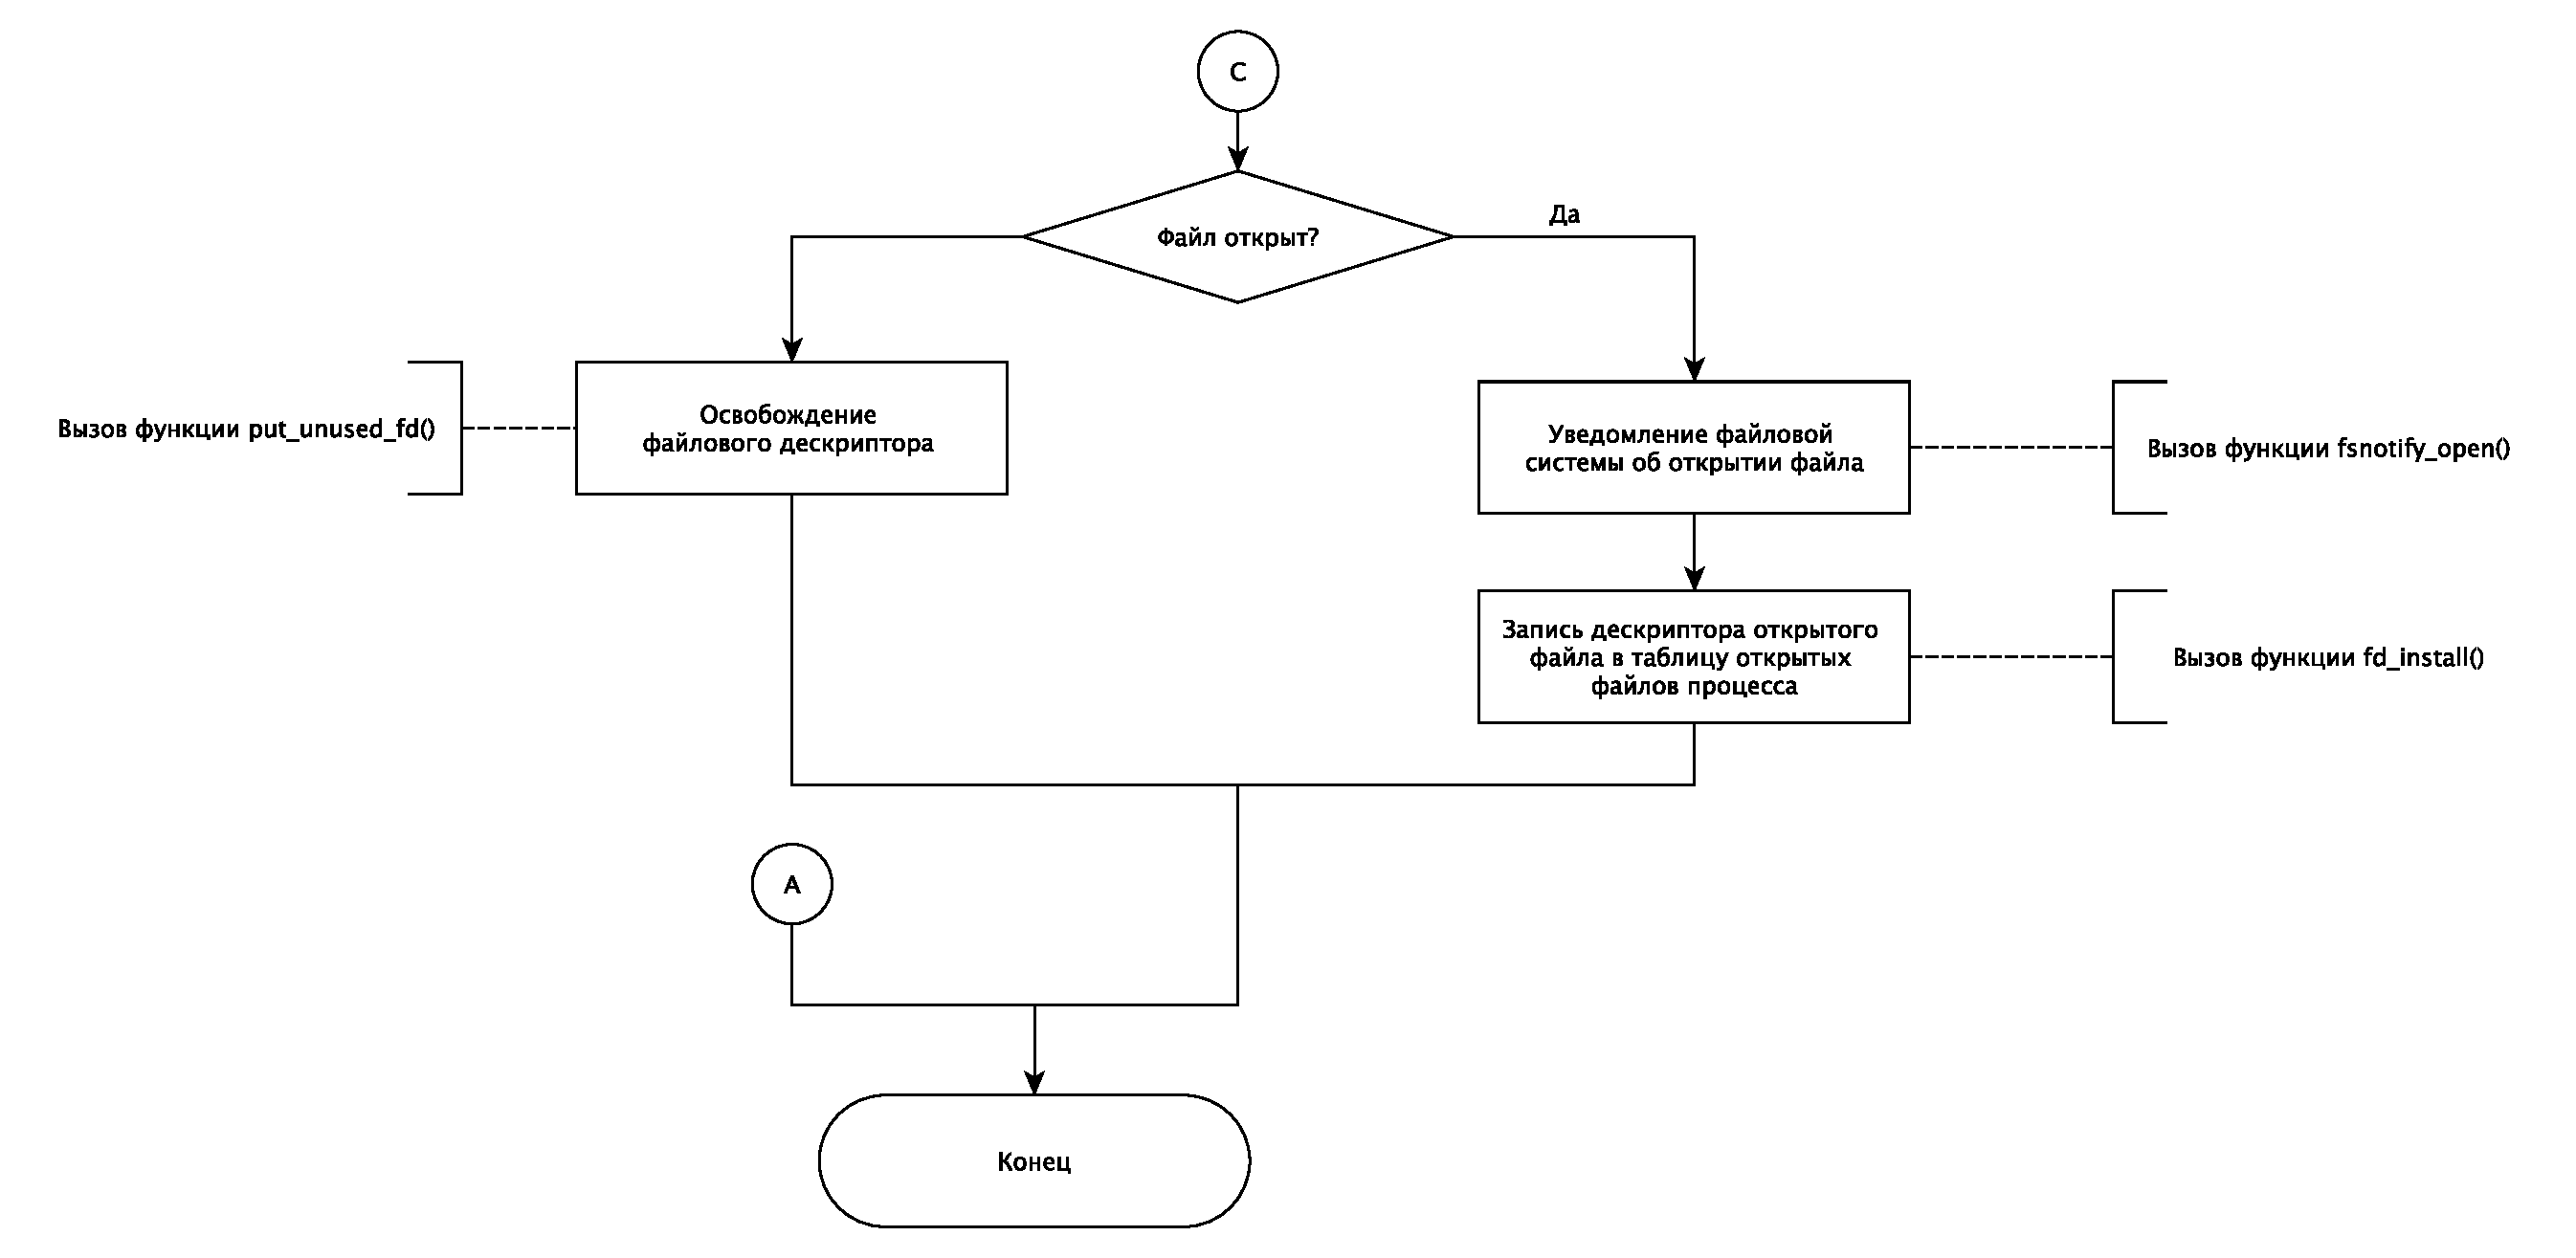
\includegraphics[scale=0.6]{3}

\item Вывод буфера сообщений ядра в стандартный поток вывода:

\includegraphics[scale=0.45]{4}

\item А выгружаем модули в обратном порядке, так как на модуль md1 ссылается некоторые другие модули или объекты ядра и до тех пор, пока число ссылок модуль в системе не станет нулевым, модуль не может быть выгружен. Модуль md2 ссылается на md1, поэтому сначала необходимо выгрузить его:

\includegraphics[scale=0.6]{7}

\includegraphics[scale=0.6]{5}

\item Функция инициализации модуля 3, выполнив все предписанные ей действия, преднамеренно возвращает ненулевое значение, что означает ошибку инициализации модуля. Этот модуль не будет подгружен к ядру, но произойдёт это уже после выполнения кода инициализирующей функции модуля в пространстве ядра:

\includegraphics[scale=0.45]{6}
\end{enumerate}

\end{document}